% !TeX root = ../main.tex
% Add the above to each chapter to make compiling the PDF easier in some editors.

\chapter{Design and Implementation}\label{chapter:design_and_implementation}
\section{Maps}	
	\subsection{Concept}
	Maps play a very important role in simulating real-world depiction of any place in the ONE simulator. This allows us to simulate the physical location as accurately as possible. The \textit{MapBased Movement} provides us with the different types of map related movements.

	The ONE Simulator requires the map in the modified Well-Known Text (WKT) Format. I call it the modified version as the WKT files utilizes points based system instead of coordinates based system. We use the Osm2Wkt tool\cite{mayer2010osm} for converting Open Street Maps (OSM) files to WKT for the ONE Simulator.

	\subsubsection {Filtering Maps}
	The ONE Simulator can accept one or more WKT map files. In case of more than 1 files, all of the files are basically overlayed on the top of each other. One thing to note is that the files need to be fully connected otherwise the ONE simulator won't start and will throw an error.

	OpenStreetMaps provides with a tool called OSMFilter \cite{osm-filter} which enables us to filter the OSM maps. This allows us to filter specific elements such as roads, bus routes etc. To use the filtered maps with ONE simulator, we need to convert each of them to WKT.

	The current implementation of the ONE simulator uses the following 4 wkt files:

	\begin{center}
    	\captionof{table}{ONE Simulator: WKT Map files used by default} \label{tab:wktMapFiles} 
	    \begin{tabular}{ | l | p{10.5cm} |}
    		\hline
    		\textbf{Map File} & \textbf{Details} \\ \hline
    		\textit{main\_roads.wkt} & represents the main roads (primary, secondary, tertiary). \\ \hline
    		\textit{roads.wkt} & represents the normal roads and streets.  \\ \hline
    		\textit{shops.wkt} & represents the shops. \\ \hline
    		\textit{pedestrian\_paths.wkt} & represents the pedestrian paths. \\ \hline
    	\end{tabular}
	\end{center}

	\subsubsection{OSM Maps}
	The first step in getting the maps is to download the OSM map from the Open Street Map export tool \cite{openstreetmap-export}. Below is a depiction of the OSM Map for Central Munich.
	\newline
	\begin{figure}[h]
		\centering
		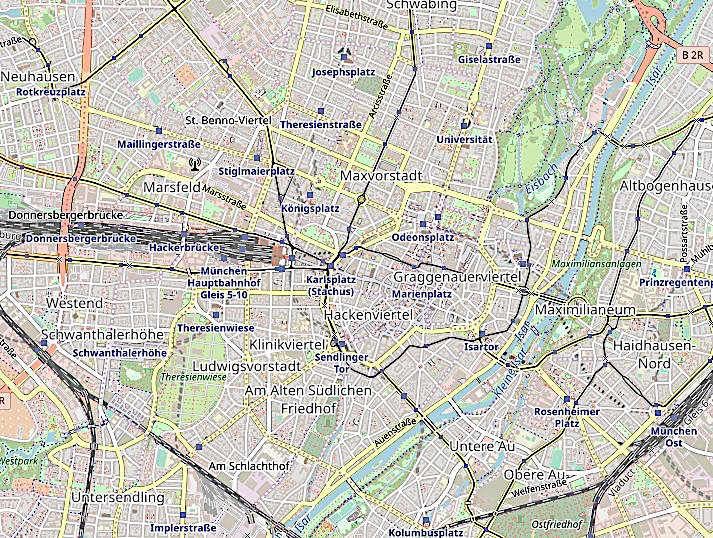
\includegraphics[scale=0.5]{./figures/central-munich-osm}
		\caption{Central Munich OSM Map - from OpenStreetMaps \cite{openstreetmap}}
	\end{figure}

	\subsubsection{Conversion to WKT}
	There are a number of tools that canconvert an OSM to WKT, however, there are a few reasons we do not use any of those tools:
	\begin{itemize}
 	 \item These tools do not make provide us with a fully connected maps. They just perform the conversion.
   	 \item These tools do not convert the coordinates to the points-based system. Even though the resulting WKT file would work with the ONE simulator, however, the distances would be very small (as compared to the original). Let me give you an example, The distance between \textit{1.0001,1.2} and \textit{1.0002,1.2} in points is \textit{11m} while if we provide this directly to the ONE simulator the distance would be \textit{0.001 m (1 mm)}.
	\end{itemize}

	\begin{figure}[h]
		\centering
		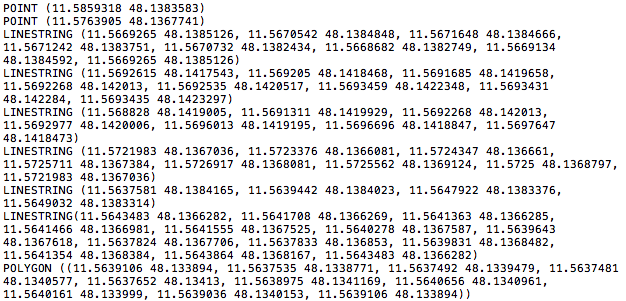
\includegraphics[scale=0.55]{./figures/wkt-file-2}
		\caption{Snapshot of WKT File Contents - Converted using OpenJump \cite{openjump} }
	\end{figure}

	We have the OSM2WKT tool \cite{mayer2010osm} as it has solution for both of the above issues and can generate a full-connected point-based WKT file that can be used with the ONE Simulator. 
	\newline
	\begin{figure}[h]
		\centering
		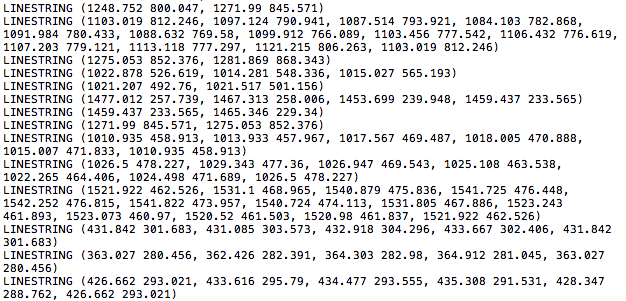
\includegraphics[scale=0.55]{./figures/wkt-file-1}
		\caption{Snapshot of WKT File Contents - Converted using OSM2WKT tool \cite{mayer2010osm} }
	\end{figure}
	\newpage
	Below is graphics depiction of the Central Munich WKT file.
	\begin{figure}[h]
		\centering
		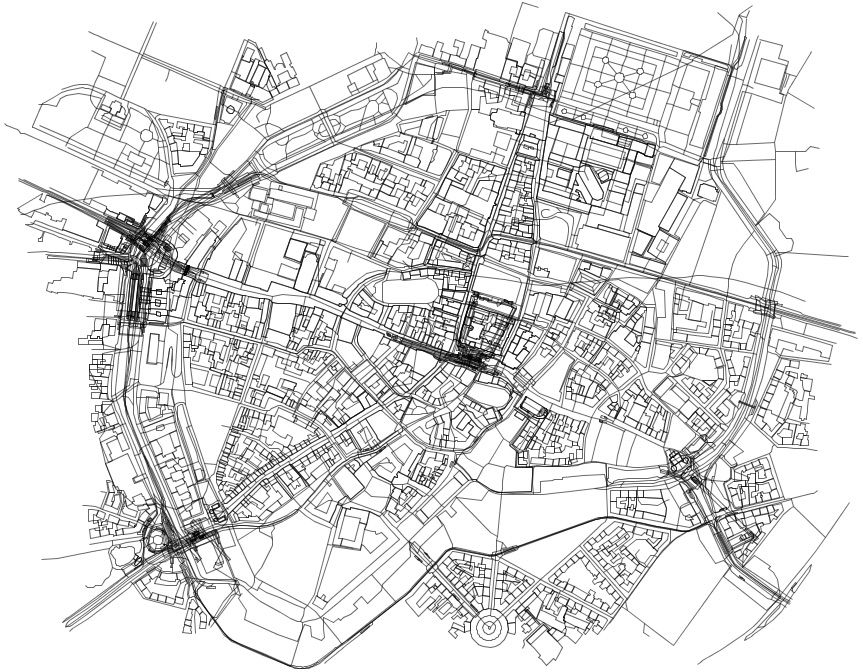
\includegraphics[scale=0.5]{./figures/central-munich-wkt}
		\caption{Central Munich WKT Map - Created using OSM2WKT tool \cite{mayer2010osm} and Screenshot using OpenJump \cite{openjump}}
	\end{figure}

\newpage
\subsection{Implementation}
\subsubsection{OSM to WKT}
Using OSM2WKT tool \cite{mayer2010osm}, any OSM file can be converted into a fully connected WKT file for use in the ONE simulator. Below are the details of how to use the OSM2WKT tool \cite{mayer2010osm} to generate a WKT file:\newline

\begin{lstlisting}[language=bash]
java -jar ./osm2wkt.jar mapfile.osm

options:
	-o outputfile - specifiying the output file. In case no outputfile is mentioned, .wkt is appended to the name of input file.
	-a - open the output file in append mode (adding the wkt output at the end of the output file)
	-t deltaX deltaY - translate map by deltaX and deltaY meters
\end{lstlisting}
\captionof{lstlisting}{Using OSM2WKT tool \cite{mayer2010osm} to generate WKT}

\vspace{8mm}
The OSM2WKT tool \cite{mayer2010osm} performs the following operations on the OSM file:
	\begin{enumerate}
 	 \item Reads the OSM Map.
   	 \item The coordinates are converted to the points based system:
   	 	\begin{enumerate}
	   	 	\item The bounding box of the map is converted into point based system (width and height in meters).
   		 	\item All the coordinates are converted to the point based system.
   		 \end{enumerate}
   	 \item The completeness of the graph is then checked and all the weird and unconnected edges are deleted so that we have a complete graph.
   	 \item The file is then saved as a WKT file.
	\end{enumerate}

\newpage
\subsubsection{Filtering OSM}
In order to filter OSM files, OSM Filter tool \cite{osm-filter} is needed. Here is the basic syntax to use the OSM Filter tool \cite{osm-filter}.
\vspace{2mm}
\begin{lstlisting}[language=bash]
	osmfilter inputfile.osm --keep="{condition}" > outputfile.osm	
\end{lstlisting}
\captionof{lstlisting}{How to use the OSM Filter tool \cite{osm-filter}}
\vspace{5mm}	

The listings below show how to create the four different types of OSM files which can then be converted to WKT files.
\vspace{5mm}	
\begin{lstlisting}[language=bash]
	osmfilter mapfile.osm --keep="highway=*ary trunk" > main_roads.osm	
\end{lstlisting}
\captionof{lstlisting}{Generating main\_roads.osm file}
\vspace{5mm}	
\begin{lstlisting}[language=bash]
	osmfilter mapfile.osm --keep="highway=residential service *link living_street"
	> roads.osm	
\end{lstlisting}
\captionof{lstlisting}{Generating roads.osm file}
\vspace{5mm}	
\begin{lstlisting}[language=bash]
	osmfilter map.osm --keep="highway=pedestrian footway living_street"
	> pedestrian_paths.osm
	
\end{lstlisting}
\captionof{lstlisting}{Generating pedestrian\_paths.osm file}
\vspace{6mm}	
\begin{lstlisting}[language=bash]
	osmfilter map.osm --keep="shop=*" > shops.osm
\end{lstlisting}
\captionof{lstlisting}{Generating shops.wkt file}
\vspace{5mm}	

The main issue with using separate osm files is that we cannot use Osm2WKT tool \cite{mayer2010osm} and it is a difficult task to make sure the resultant map is fully connected. I have modified the Osm2WKT tool \cite{mayer2010osm} to accept more than 1 OSM files and generate the corresponding WKT files that are fully connected, however, that is beyond the scope of this document. In our simulations, we are using a single map file.

\subsection{Configuration}
In order to utlize the MapBasedMovement and the map files we have prepared (using method in the above sections), we would need to add the following to one of the configuration files:\newline

\begin{lstlisting}[language=bash]
Group.movementModel = MapBasedMovement

# Configuration for 1 map file
MapBasedMovement.nrofMapFiles = 1
MapBasedMovement.mapFile1 = data/maps/map.wkt


# Configuration for multiple maps files (these files need to be connected (when overlayed on each other))
MapBasedMovement.nrofMapFiles = 4

MapBasedMovement.mapFile1 = data/maps/roads.wkt
MapBasedMovement.mapFile2 = data/maps/main_roads.wkt
MapBasedMovement.mapFile3 = data/maps/pedestrian_paths.wkt
MapBasedMovement.mapFile4 = data/maps/shops.wkt

\end{lstlisting}
\captionof{lstlisting}{Map-based Movement Configuration}
\newpage

\section{Access Points}
\subsection{Concept}
Access Points are devices that connect devices to one another and facilities the flow of information among devices. An Access Point can operate in any of the following three modes:

	\begin{center}
    	\captionof{table}{ONE Simulator: Modes of Operation for Access Points/Wifi Interface} 
	    \begin{tabular}{ | l | p{10.5cm} |}
    		\hline
    		\textbf{Mode} & \textbf{Description} \\ \hline
    		\textit{Access Point (AP)} & Access Point (AP) provides a bridge for two Station Adapters (SAs) to connect and communicate with each other. Two Access Points cannot talk to each other directly. \\ \hline
    		\textit{Station Adapter (SA)} & Station Adapter (SA) is a passive device that can connect to an Access Point and communicate to other Station Adapters using the Access Point (AP). Two Station Adapters cannot talk to each other directly. \\ \hline
    		\textit{Adhoc} & Adhoc Mode is used when we want two devices to connect and communicate direclty to each other. Hosts in Adhoc mode cannot connect to either an Access Point (AP) or Station Adapter(SA) and vice versa. This is the default mode.\\ \hline
    	\end{tabular}
	\end{center}
	\vspace{3mm}
	\begin{figure}[h]
		\centering 
		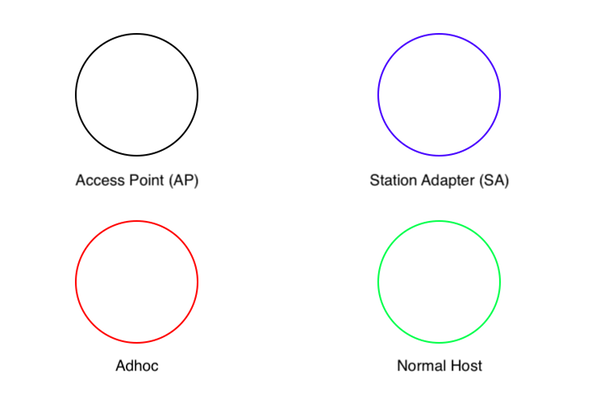
\includegraphics[scale=0.45]{./figures/aps-1}
		\caption{Hosts with Access Points (SA, AP and Adhoc) and Normal Host}
	\end{figure}
	\newpage
	The above coloring combination is used in the ONE Simulator to give user the ability to visually different between the hosts with different modes (or no mode at all). Below is a screenshot from the ONE Simulator with all of the above Hosts in action.
	\begin{figure}[h]
		\centering
		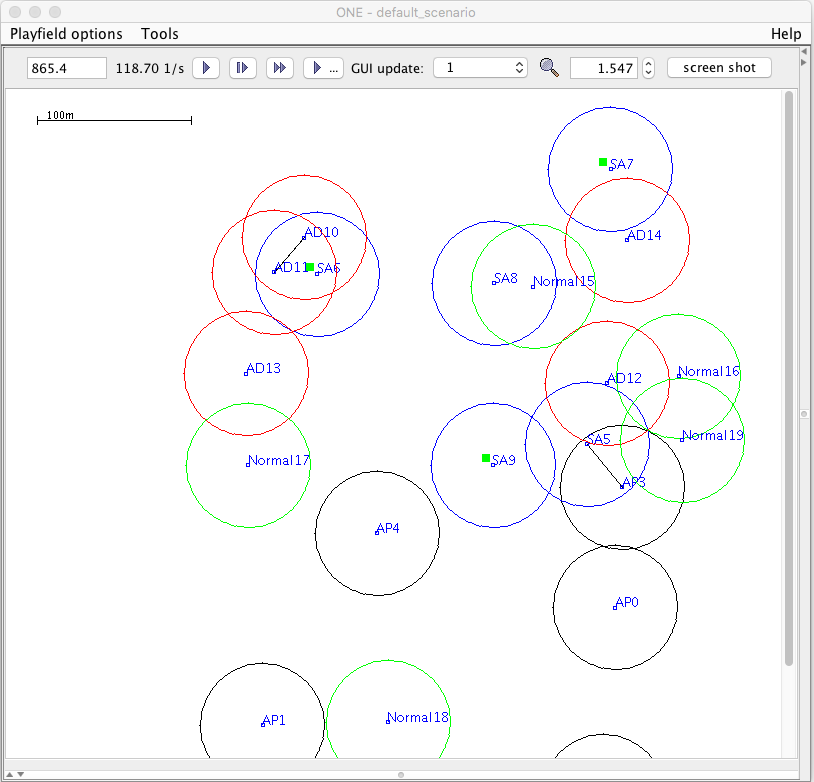
\includegraphics[scale=0.5]{./figures/aps-2}
		\caption{ONE Simulator showing all the Hosts (AP enabled and normal) in action}
	\end{figure}
\newpage
\subsection{Implementation}
Before discussing implementation details, I would like to discuss the pre-requisite for the implementation. The following table lists two classes and what they are used for:
	\begin{center} 
	    \begin{tabular}{ | l | p{10.5cm} |}
    		\hline
    		\textbf{Class} & \textbf{Description} \\ \hline
    		\textit{DTNHost} & This class represents a DTN Capable host. It contains all the properties and functionalities fo the host such as groupID, MessageListeners, MovementListeners etc. \\ \hline
    		\textit{DTNHostWithWifi} & This class is a subclass of the \textit{DTNHost} class and represents a host with Access Point/Wifi capability. It inherits everything from the parent class and adds an extra mode (which can either be ADHOC, AP or SA). \\ \hline
    	\end{tabular}
       	\captionof{table}{ONE Simulator: Classes related to Hosts/Nodes} 
	\end{center}
\vspace{3mm}
\textit{DNTHostWithWifi} is a very lean host that takes everything from its parent \textit{DTNHost} and adds the mode. The following listing shows the implementation of \textit{DTNHostWithWifi}.
\begin{lstlisting}[language=java]
public class DTNHostWithWifi extends DTNHost {
	public static int AP = 1;
	public static int SA = 2;
	public static int ADHOC = 3;
	private int mode;

	public DTNHostWithWifi(List<MessageListener> msgLs, List<MovementListener> movLs, String groupId,List<NetworkInterface> interf, ModuleCommunicationBus comBus, MovementModel mmProto, MessageRouter mRouterProto, String mode) {	
		super(msgLs, movLs, groupId, interf, comBus, mmProto, mRouterProto);	
		this.mode = mode.equalsIgnoreCase("ap") ? AP : mode.equalsIgnoreCase("sa") ? SA : ADHOC;
	}
	public int getMode() {
		return mode;
	}
	public String getModeName() {		
		return mode == ADHOC ? "ADHOC" : (mode == AP ? "AP" : "AP");
	}
}
\end{lstlisting}
\captionof{lstlisting}{ONE Simulator: DTNHostWithWifi Implementation}
\vspace{5mm}
There is still another component that needs to be implemented i.e. an interface to the new \textit{DTNHostWithWifi}. We call it \textit{WifiInterface}. The following table discusses the two main classes.

\begin{center}
    	\captionof{table}{ONE Simulator: WifiInterface \& its parent interface} 
	    \begin{tabular}{ | l | p{10cm} |}
    		\hline
    		\textbf{Class} & \textbf{Description} \\ \hline
    		\textit{SimpleBroadcastInterface} & \textit{SimpleBroadcastInterface} is a Network Interface that is responsible for connectivity among hosts. It allows one-to-one transmissions with a constant bit-rate.\\ \hline
    		\textit{WifiInterface} & \textit{WifiInterface} is responsible for connectivity between two different \textit{DTNHostWithWifi} objects. It is also responsible that the connection rules (SA can connect only to AP, Adhoc hosts can connect to each other only) are upheld. \\ \hline
    	\end{tabular}
	\end{center}
\vspace{3mm}
\textit{WifiInterface} takes almost everything from its parent but adds the extra ability to check if two \textit{DTNHostWithWifi} can connect to each other. Another method that it overrides is the ability to return \textit{DTNHostWithWifi} with the \textit{getHost()} method.
\vspace{3mm}

\begin{lstlisting}[language=java]
public class WifiInterface extends SimpleBroadcastInterface {
	...	 
	public void connect(NetworkInterface anotherInterface) {
		if (canConnectTo(anotherInterface)) {
			...
		}
	}

	/*
	 * Along with the usual connectivity rules, we also check if the 
	 * DTNHosts can connect to each other by having compatible modes.
	 */
	boolean canConnectTo(NetworkInterface anotherInterface) {
		boolean canConnect = isScanning()  
		&& anotherInterface.getHost().isRadioActive() 
		&& isWithinRange(anotherInterface) 
		&& !isConnected(anotherInterface)
		&& (this != anotherInterface);
		
		if(canConnect) {
			WifiInterface thisInterface = (WifiInterface) this;
			WifiInterface secondInterface = (WifiInterface) anotherInterface;
			
			int thisInterfaceMode = thisInterface.getHost().getMode();
			int secondInterfaceMode = secondInterface.getHost().getMode();

			if(thisInterfaceMode == DTNHostWithWifi.ADHOC) {
				canConnect = thisInterfaceMode == secondInterfaceMode;				
			} else {
				canConnect = (thisInterfaceMode == DTNHostWithWifi.AP && secondInterfaceMode == DTNHostWithWifi.SA) 
				|| (thisInterfaceMode == DTNHostWithWifi.SA && secondInterfaceMode == DTNHostWithWifi.AP);
			}
		}
		
		return canConnect;
	}	
	
	public DTNHostWithWifi getHost() {
		return (DTNHostWithWifi)host;
	}
}
\end{lstlisting}
\captionof{lstlisting}{ONE Simulator: WifiInterface Implementation}
\newpage

Now, we need to combine both of these to make sure that any host having a \textit{WifiInterface} is instantiated as \textit{DTNHostWithWifi} objects and all othe other hosts are instantiated as \textit{DTNHost} objects. This needs to be done inside \textit{createHosts()} function of \textit{SimScenario} class. Below are the changes that are made to achieve this purpose:
vspace{3mm}
\begin{lstlisting}[language=java]
			boolean hasWifiInterface = false;
			
			// setup interfaces
			for (int j=1;j<=nrofInterfaces;j++) {
				...
				if(iface instanceof WifiInterface) {
					hasWifiInterface = true;
				}
				...
			}
			...
			//Get Wifi modes for hosts (only exist for DTNHostWithWifi)
			List<String> modes = new ArrayList<String>();
			String wifiMode = s.getSetting("mode",null);

			if(wifiMode == null) {
				String modesFile = s.getSetting("modesFile",null);
				if(modesFile != null) {
					try {
						Scanner in = new Scanner(new FileReader(modesFile));
						while(in.hasNextLine()) {
							modes.add(in.nextLine());
						}
						in.close();
					} catch (FileNotFoundException e) {}
				}
			}
			
			// creates hosts of ith group
			for (int j=0; j<nrofHosts; j++) {
				...
				if(!hasWifiInterface) {
					DTNHost host = new DTNHost(this.messageListeners, 
						this.movementListeners,	gid, interfaces, comBus, 
						mmProto, mRouterProto);
					hosts.add(host);
				} else {
					String mode = wifiMode != null ? wifiMode : (j < modes.size() ? modes.get(j) : "");
				
					DTNHostWithWifi host = new DTNHostWithWifi(this.messageListeners, this.movementListeners, gid, interfaces, comBus, mmProto, mRouterProto,  mode: mode);
					hosts.add(host);
				}
			}
		}
	}
\end{lstlisting}
\captionof{lstlisting}{ONE Simulator: Changes to SimScenario for Implementation of the AP-capable hosts}
\subsection{Configuration}
Here we will show how to configure \textit{DTNHost} and \textit{DTNHostWithWifi}. We will also show how to configure \textit{mode} for \textit{DTNHostWithWifi}.

\begin{lstlisting}[language=bash]
# We need to create two different types of interfaces (based on the types of interface, either DTNHost or DTNHostWithWifi object is created)

# Declaring WifiInterface (any host/group of hosts having this interface will be the DTNHostWithWifi hosts)
wifiInterface.type = WifiInterface
wifiInterface.transmitSpeed = 50k
wifiInterface.transmitRange = 40

# Declaring SimpleBroadcastInterface (any host/group of hosts having this interface will be the DTNHost hosts)
btInterface.type = SimpleBroadcastInterface
btInterface.transmitSpeed = 250k
btInterface.transmitRange = 10

# Making sure all the groups are counted and created
Scenario.nrofHostGroups = 5


# Defining general behavior for Groups
Group.nrofInterfaces = 1
Group.interface1 = btInterface

# Defining normal DTNHosts (We do not need to attach btInterface as all the groups would have the btInterface by default)
Group1.groupID = Normal

# Defining Station Adapters (groupID can be anything as only the mode can identify between different types of hosts)
Group2.groupID = SA           
Group2.interface1 = wifiInterface
Group2.mode = sa

# Defining Access Points
Group3.groupID = AP
Group3.interface1 = wifiInterface
Group3.mode = ap

# Defining Adhoc nodes (We can eliminate mode here as well as adhoc is the default mode)
Group4.groupID = ADHOC
Group4.interface1 = wifiInterface
Group4.mode = adhoc

# Declearing Wifi nodes with different modes (modes are contained in the modesFile)
Group5.groupID = D
Group5.interface1 = wifiInterface
Group5.modesFile = data/modes.txt   #modes.txt is containing one mode per line. The mode is applied to the hosts in the same order

\end{lstlisting}
\newpage
\section{Snapping to Access Points}
\subsection{Concept}
In the \hyperref[section:floating-content]{\emph{Floating Content Section}}, it was discussed that a message is tagged with geographical coordinates and an availability/radius. \textit{Snapping to Access Point} is the concept of increasing the availability of the message beyond its original availability zone. In the configuration, we can define how many Access Points should the message snap to at maximum. Theoretically, the number of snapped Access Points should directly influence the TTL (Time to live) of the message. Below is a step-wise explanation of the process:

	\begin{enumerate}
 	 \item The host Station Adapter (\textit{SA1}) generates a message \textit{M} with a center \textit{C} (which is the location of \textit{SA1} at that time), availability \textit{a} and number of maximum access points to snap to (\textit{k}). Assuming \textit{k = 3}.
 	 \item \textit{SA1} comes in contact with an Access Point (\textit{AP1}), connection is made and a copy of the message \textit{M} is transferred (\textit{M'}).
 	 \item If \textit{k}-value for the original message \textit{M} is greater than 0:
 	 	\begin{enumerate}
 	 		\item \textit{k}-value for the original message (\textit{M}) is decreased by 1.
 	 		\item \textit{k}-value for the copied message (\textit{M'}) is set to zero.
 	 		\item The center of the copied message (\textit{M'}) is changed to the center of the Access Point (\textit{AP1}).
 	 	\end{enumerate}
 	 \item The above process continues for the original message \textit{M} until \textit{k}=0. 	 		
 	 \end{enumerate}
 	 
 	Since the ID of the message \textit{M} and all of the copies is the same, they are treated as the same message; which allows us to extend the availability of the message.  \newline
 	There are a few important points to note:
	\begin{enumerate}
 	 \item Copies of the message are not snapped to any access point, Only the original message is snapped.
 	 \item If a message is snapped to 1 access point which drops it due to any reason (apart from TTL expiry), whenever that message (the original or even the copy which knows about this access point) is copied again, it is snapped to that access point again.
 	 \item The availability zones of the copies might or might not intersect each other, however, the availability zone of the original message and each copy would have an overlap.
 	 \end{enumerate}
	\begin{figure}[h]
		\centering 
		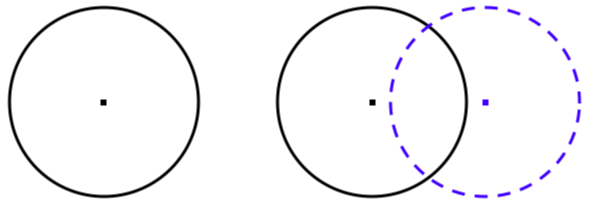
\includegraphics[scale=0.45]{./figures/snapped-to-ap-1}
		\caption{Availability zones of Message with k=0 (not snapped yet) to the left and k=1 (snapped to 1 Access Point) to the right}
	\end{figure}
	\vspace{8mm}
	\begin{figure}[h]
		\centering 
		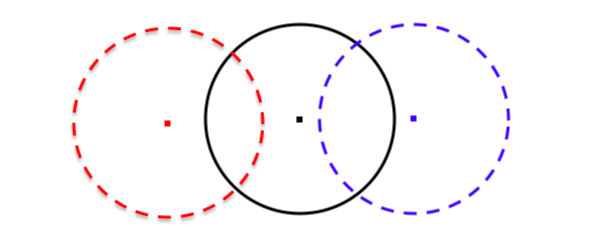
\includegraphics[scale=0.45]{./figures/snapped-to-ap-2}
		\caption{Availability zones of Message with k=2 (snapped to 2 Access Points)}
	\end{figure}
	\vspace{5mm}
	\begin{figure}[h!]
		\centering 
		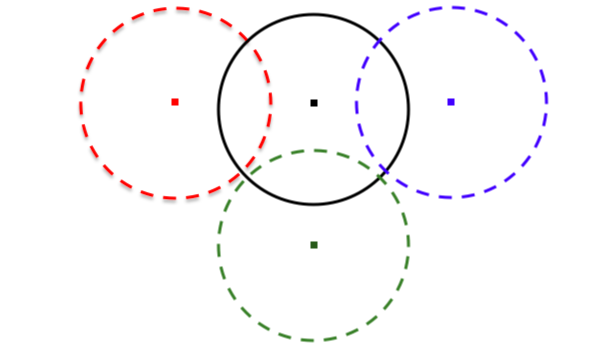
\includegraphics[scale=0.45]{./figures/snapped-to-ap-3}
		\caption{Availability zones of Message with k=3 (snapped to 3 Access Points)}
	\end{figure}
	\begin{figure}[h!]
		\centering 
		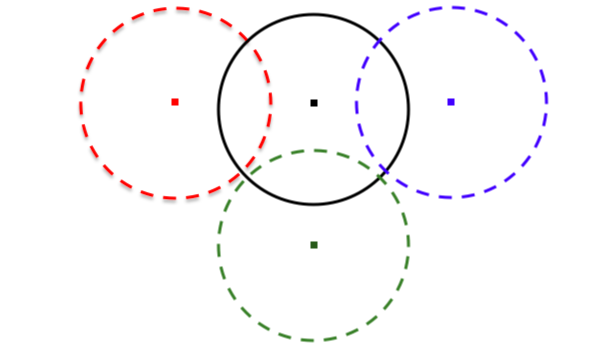
\includegraphics[scale=0.45]{./figures/snapped-to-ap-4}
		\caption{Special Case: Message with k=3 where there is no overlap between availability zones of the copies}
	\end{figure}

\newpage
\subsection{Implementation}
\subsubsection{Snapping to Access Point}
\begin{enumerate}
	\item The very first point is to attach an \textit{originalAnchor} to the message (which is the point where the message was originally generated).		
	\begin{lstlisting}[language=java]
	m.addProperty("originalAnchor", m.getProperty("anchor"));
	\end{lstlisting}
	\item The settings for the number of Access Points to snap to (\textit{kNextAPs}) is fetched inside \textit{FloatingContentRouter}.
	\begin{lstlisting}[language=java]
		if (fcSettings.contains(FC_NUM_OF_APS))
			kNextAPs = fcSettings.getInt(FC_NUM_OF_APS);
	\end{lstlisting}
	\item When message transfer is complete (\textit{messageTransferred} method in \textit{FloatingContentRouter}), we need to check f the message need to be snapped to any Access Point (by checking \textit{kNextAPs} property of the message).:
	\begin{enumerate}
		\item If the host does not have a wifi interface, the control is returned back to the caller.
		\begin{lstlisting}[language=java]
			if(!(this.getHost() instanceof DTNHostWithWifi)
				return m;
			\end{lstlisting}
		\item If the receiving node is not an access point, the control is returned back to the caller.
		\begin{lstlisting}[language=java]
			DTNHostWithWifi receivingNode = (DTNHostWithWifi) this.getHost();
			if(receivingNode.getMode() != DTNHostWithWifi.AP)
				return m;
		\end{lstlisting}

		\item \textit{kNextAP} for the copied message is set to 0.
		\begin{lstlisting}[language=java]
			m.updateProperty(FC_NUM_OF_APS, 0);
		\end{lstlisting}

		\item The \textit{anchor} of the copy is set to location of the access point if the message had been already anchored to this access point and the message still can be anchored to access points (\textit{kNextAPs>0}). Decrease \textit{kNextAPs} only if the message was not previously anchored to this access point.
		\begin{lstlisting}[language=java]
		if ((int) msg.getProperty(FC_NUM_OF_APS) > 0 || (anchorAccessPoints != null && anchorAccessPoints.contains(receivingNode.toString()))) {
			m.updateProperty(FC_ANCHOR, receivingNode.getLocation().clone());

			if((int) msg.getProperty(FC_NUM_OF_APS) > 0)
				msg.updateProperty(FC_NUM_OF_APS, (int) msg.getProperty(FC_NUM_OF_APS) - 1);
		}
		\end{lstlisting}
		\item The access point ID is added to the list of APS (\textit{anchorAPs}) property of the message. This helps us in re-snapping the message to the access point if the access points get a new copy of the same message.
		\begin{lstlisting}[language=java]
		anchorAccessPoints.add(receivingNode.toString());				
		msg.updateProperty(FC_ANCHOR_APS, anchorAccessPoints);
		m.updateProperty(FC_ANCHOR_APS, anchorAccessPoints);
		\end{lstlisting}
		\item The access point location is added to the list of APS (\textit{anchorAPsLocation}) property of the message. This is used to make sure that the new availability zones are also accounted for before trying to delete a message.
		\begin{lstlisting}[language=java]
		anchorAccessPointsLocations.add(receivingNode.getLocation().clone());
		msg.updateProperty(FC_ANCHOR_APS_LOC, anchorAccessPointsLocations);
		m.updateProperty(FC_ANCHOR_APS_LOC, anchorAccessPointsLocations);
		\end{lstlisting}
		\end{enumerate}
\end{enumerate}
\subsubsection{Changes to Message Deletion Algorithm}
Here we are making sure that the message is deleted only after the it is outside of the new availability zones (in case a message is snapped to access point, we need to check that the message is outside all the availability zones for that message).

\begin{lstlisting}[language=java]
for (Message m : m_set) {
	ArrayList<Coord> locations;
	try {
		locations = new ArrayList<Coord>((HashSet<Coord>)m.getProperty(FloatingContentRouter.FC_ANCHOR_APS_LOC));
	} catch(NullPointerException ignored) {
		locations = new ArrayList<>();						
	}

	locations.add(0, (Coord)m.getProperty(FC_ANCHOR));
	locations.add(1,(Coord)m.getProperty(FC_ANCHOR_ORIGINAL));
		
	int counter = 0;
	while(counter<locations.size()) {
		distance_curr = loc.distance(locations.get(counter));
		
		if ((deletion_check(distance_curr, (Double) m.getProperty(FC_R), (Double) m.getProperty(FC_A)) != 1))
				break;
		counter ++;
	}
					
	if(counter == locations.size() && !d_list.contains(m.getId()))
		d_list.add(m.getId());
}
\end{lstlisting}
\subsection{Configuration}
\begin{lstlisting}[language=bash]
FloatingContentRouter.kNextAPs = 1
\end{lstlisting}
\newpage
\section{Access Points Data}
\subsection{Concept}
\subsubsection{Data Collection}
We are using the wifi access points database from RadioCells \cite{wifi-data}. The database has a number of tables, however, we are only concerned with \textit{wifi\_zone}. We are only using \textit{latitude} and \textit{longitude} data.
\subsubsection{Data Processing}
We follow the following steps to process the data for the ONE Simulator:
\begin{enumerate}
	\item The data from sqlite database is exported to a text file. 
	\item The data is processed by removing the double quotes and separating latitude and longitude by a comma (,).
	\item To make sure that the coordinates are converted to the correct scaling, we add the boundary coordinates to the file. Below are the boundary coordinates:
	\begin{itemize}
		\item minimumLatitude,0
		\item maximumLatitude,0
		\item 0,minimumLongitude
		\item 0,maximumLongitude
	\end{itemize}
	\item The processed file is then passed to a Coordinate Converter which returns a WKT file with the transformed coordinates.
	\item The WKT file can then be used for setting up the access points on the map using \textit{StationaryMapBasedMovement}.
\end{enumerate}
\begin{figure}[h]
	\centering
	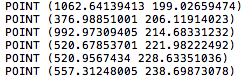
\includegraphics{./figures/access-points-data}
	\caption{Transformed Access Points Data}
\end{figure}
\subsection{Implementation}
A majority of the implementation is taken from Osm2Wkt \cite{mayer2010osm}. The implementation is pretty straight-forward and can be explained in the following steps:
\begin{enumerate}
\item We open the file and read the content into an array of Landmarks (\textit{Landmark} has \textit{latitude}, \textit{longitude} for the original coordinates as well as \textit{x}, \textit{y} for storing the transformed coordinates)
\begin{lstlisting}[language=java]
Scanner in = new Scanner(new FileReader(filePath));

while(in.hasNextLine()) {
	String text = in.nextLine().trim();
	if(text.length() > 0) {
		String[] coordinates = text.split(",");
		Landmark landmark = new Landmark(Double.parseDouble(coordinates[0]), Double.parseDouble(coordinates[1]));
		landmarks.add(landmark);
	}
}
in.close();
\end{lstlisting}
\item The coordinates are then transformed using \textit{transformCoordinates} \cite{mayer2010osm}.
\item Finally the coordinates are written in a WKT file which can be used by the ONE Simulator.
\end{enumerate}

To Read the WKT file in ONE simulator, we have implemented \textit{StationaryMapBasedMovement} and \textit{MapNodeExtended} classes. The following table explains the functionality of each of these classes.

	\begin{center}
	    \begin{tabular}{ | l | p{8.8cm} |}
    		\hline
    		\textbf{Class} & \textbf{Details} \\ \hline
    		\textit{MapNodeExtended} & Inherits from the \textit{MapNode} class. It reads the WKT file and apply transformations (mirror and translation) to the location points. \\ \hline
    		\textit{StationaryMapBasedMovement} & Inherits from \textit{MapBasedMovement} class. Get list of transformed locations (from the WKT file) by passing it to \textit{MapNodeExtended}. \\ \hline
    	\end{tabular}
    	\captionof{table}{ONE Simulator: Classes for WKT based Node positioning} \label{tab:wktMapFiles} 

	\end{center}
\newpage
Below are two main functions from \textit{StationaryMapBasedMovement}.
\vspace{3mm}
\begin{lstlisting}[language=java]
	public StationaryMapBasedMovement(Settings settings) {
		super(settings);

		String fileName = settings.getSetting(ROUTE_FILE_S);
		allNodes = MapNodeExtended.readNodes(fileName, getMap());		
	}
		
	@Override
	public Coord getInitialLocation() {
		counter = (counter + 1) \% allNodes.size();
		return allNodes.get(counter).getLocation();
	}
\end{lstlisting}
\captionof{lstlisting}{Main features of \textit{StationaryMapBasedMovement} class}

\vspace{10mm}
Below is the main code snippet from \textit{MapNodeExtended} class.
\vspace{3mm}
\begin{lstlisting}[language=java]
		WKTReader reader = new WKTReader();
		List<Coord> coords;
		File routeFile = null;
		
		double xOffset = map.getOffset().getX();
		double yOffset = map.getOffset().getY();

		List<MapNode> nodes = new ArrayList<MapNode>();

		try {
			routeFile = new File(fileName);
			coords = reader.readPoints(routeFile);
		}
		catch (IOException ioe) {
			throw new SettingsError("Couldn't read MapRoute-data file " + 
					fileName + 	" (cause: " + ioe.getMessage() + ")");
		}


		for (Coord c : coords) {			
			if(map.isMirrored())
				c.mirror();
			
			c.translate(xOffset, yOffset);
			
			MapNode node = map.getNodeByCoord(c);
			if (node == null) {
				node = new MapNode(c);
			}
			nodes.add(new MapNodeExtended(node));			
		}
		
		return nodes;
\end{lstlisting}
\captionof{lstlisting}{Getting List of all MapNodes (taken from \textit{MapNodeExtended})}
\vspace{8mm}
\subsection{Configuration}
\begin{lstlisting}[language=bash]
Group1.routeFile = data/path_to_wkt_file/file_name.wkt
\end{lstlisting}